% AcademiX - Presentacion Entrega 1
% Compilar con pdfLaTeX (Overleaf: Menu > Compiler > pdfLaTeX).
% Duracion objetivo: 10 minutos de exposicion + preguntas.
% Guion sugerido (13 laminas de cuerpo): titulo 20s | problema 60s | valor 60s |
% interesados 45s | necesidades 60s | riesgos 60s | alcance RF 70s | RNF 70s |
% stack y decisiones abiertas 60s | arquitectura 50s | maquetas 50s | plan 50s | cierre 30s.
% Las laminas posteriores a \appendix son respaldo para preguntas: no se exponen.
\documentclass[aspectratio=169,10pt]{beamer}

\usetheme{Boadilla}
\usepackage[utf8]{inputenc}
\usepackage[T1]{fontenc}
\usepackage[spanish,es-noshorthands]{babel}
\usepackage{graphicx}
\usepackage{tabularx}
\usepackage{booktabs}
\usepackage{xcolor}
\usepackage{tikz}

\usetikzlibrary{arrows.meta,positioning}

\definecolor{academixnavy}{HTML}{1E3A5F}
\definecolor{academixamber}{HTML}{A16207}
\definecolor{academixbg}{HTML}{F8FAFC}
\definecolor{academixline}{HTML}{CBD5E1}
\definecolor{academixslate}{HTML}{64748B}

\setbeamercolor{structure}{fg=academixnavy}
\setbeamercolor{frametitle}{fg=academixnavy,bg=academixbg}
\setbeamercolor{title}{fg=academixnavy}
\setbeamercolor{block title}{fg=white,bg=academixnavy}
\setbeamercolor{block body}{fg=black,bg=academixbg}
\setbeamercolor{alerted text}{fg=academixamber}
\setbeamertemplate{navigation symbols}{}
\setbeamertemplate{itemize item}{\color{academixamber}$\blacktriangleright$}
\setbeamertemplate{itemize subitem}{\color{academixnavy}$\bullet$}
\setbeamertemplate{footline}[frame number]
\setbeamerfont{frametitle}{size=\large}

\newcolumntype{Y}{>{\raggedright\arraybackslash}X}
\newcommand{\st}[1]{\textcolor{academixamber}{\textbf{#1}}}

\title[AcademiX]{AcademiX}
\subtitle{LMS multi-tenant universitario}
\author[Equipo Lock In]{Equipo Lock In}
\institute[IIC3143]{IIC3143 Desarrollo de Software}
\date{Entrega 1}

\begin{document}

% --- Titulo (20 s) ---
\begin{frame}
  \titlepage
  \vspace{-0.5cm}
  \centering
  \small Curso $\rightarrow$ módulos $\rightarrow$ material $\rightarrow$ evaluaciones $\rightarrow$ entregas $\rightarrow$ corrección $\rightarrow$ notas
\end{frame}

% --- 1. Problema (60 s) ---
\begin{frame}{1. Problema y justificación}
\begin{block}{Contexto}
Los LMS centralizan el curso, pero el flujo académico real termina repartido entre la plataforma institucional, planillas, correos, calendarios externos y carpetas de archivos.
\end{block}
\begin{itemize}
  \item El estudiante no distingue rápido qué estudiar, qué entregar y qué notas ya salieron.
  \item El cuerpo docente administra ponderaciones, corrección y publicación con herramientas externas.
  \item La institución necesita continuidad, seguridad y aislamiento de datos por universidad.
\end{itemize}
\vspace{0.1cm}
\begin{block}{Principio fundamental}
\footnotesize Los flujos principales de un curso deben poder completarse dentro de la plataforma, sin depender de planillas, carpetas, calendarios o canales externos.
\end{block}
\end{frame}

% --- Valor de negocio (60 s) ---
\begin{frame}{Valor de negocio}
\begin{columns}[T,onlytextwidth]
\begin{column}{0.48\textwidth}
\begin{block}{Dolor actual}
\begin{itemize}
  \item Experiencia académica fragmentada.
  \item Notas y ponderaciones fuera de la plataforma.
  \item Material pasivo, desconectado de la evaluación.
  \item Riesgo justo en cierres de entrega y publicación.
\end{itemize}
\end{block}
\end{column}
\begin{column}{0.48\textwidth}
\begin{block}{Valor propuesto}
\begin{itemize}
  \item Flujo académico integrado en un solo lugar.
  \item Evidencia y trazabilidad de entregas y notas.
  \item Cálculo de promedios y liberación controlada.
  \item Arquitectura lista para varias universidades.
\end{itemize}
\end{block}
\end{column}
\end{columns}
\vspace{0.2cm}
{\footnotesize Se busca una integración del flujo académico crítico, más que un posicionarse en paridad funcional con plataformas como Canvas o Moodle.}
\end{frame}

% --- 2. Interesados y usuarios (45 s) ---
\begin{frame}{2. Interesados y usuarios}
\small
\begin{tabularx}{\textwidth}{lYY}
\toprule
\multicolumn{3}{l}{\textbf{Interesados} (afectados por el resultado)} \\
\midrule
Universidad & Continuidad, seguridad y control de sus datos & Opera o contrata el LMS \\
Departamento académico & Periodos, cursos, secciones y equipos docentes & Coordina la oferta del semestre \\
Equipo técnico & Arquitectura desplegable y observable & Construye y evoluciona \\
\midrule
\multicolumn{3}{l}{\textbf{Usuarios} (operan el sistema; rol según tenant y curso)} \\
\midrule
Administrador de tenant & Usuarios, periodos, cursos e inscripciones & Gestiona la institución \\
Docente & Material, evaluaciones, corrección y calificaciones & Configura y publica \\
Ayudante & Corrección, comentarios y apoyo operativo & Ejecuta tareas delegadas \\
Estudiante & Cursos, pendientes, cuerpo docente y notas liberadas & Usa el flujo diario \\
\bottomrule
\end{tabularx}
\end{frame}

% --- 3. Necesidades (60 s) ---
\begin{frame}{3. Necesidades que resuelve AcademiX}
\small
\begin{itemize}
  \item \textbf{Claridad diaria:} dashboard con cursos, próximas evaluaciones y anuncios.
  \item \textbf{Cuerpo docente visible:} el estudiante identifica por nombre y rol a quién responde por su sección.
  \item \textbf{Material organizado:} módulos publicados u ocultos, con archivos y enlaces.
  \item \textbf{Evaluaciones trazables:} fecha, puntaje, ponderación, entrega y estado.
  \item \textbf{Calificación transparente:} promedios calculados según ponderaciones y liberación manual.
  \item \textbf{Aislamiento institucional:} cada universidad opera como tenant separado.
\end{itemize}
\vspace{0.1cm}
\begin{columns}[T,onlytextwidth]
\begin{column}{0.49\textwidth}
\begin{block}{Fundaciones y extensiones}
\footnotesize Fundaciones \emph{must have}: cursos y secciones, participantes, cuerpo docente visible, evaluaciones y calificaciones. Fundaciones \emph{nice to have}: Video, IA, chats, calendario y alertas: sólo después de validar las fundaciones.
\end{block}
\end{column}
\begin{column}{0.49\textwidth}
\begin{block}{Suposiciones}
\footnotesize Se asume un Tenant por universidad, un curso equivale a un ramo semestral. Se contemplan 5 universidades de hasta 30.000 estudiantes cada una.
\end{block}
\end{column}
\end{columns}
\end{frame}

\begin{frame}{Modelos de Proceso: Corrección y publicación}
\begin{columns}[T,onlytextwidth]
\begin{column}{0.62\textwidth}
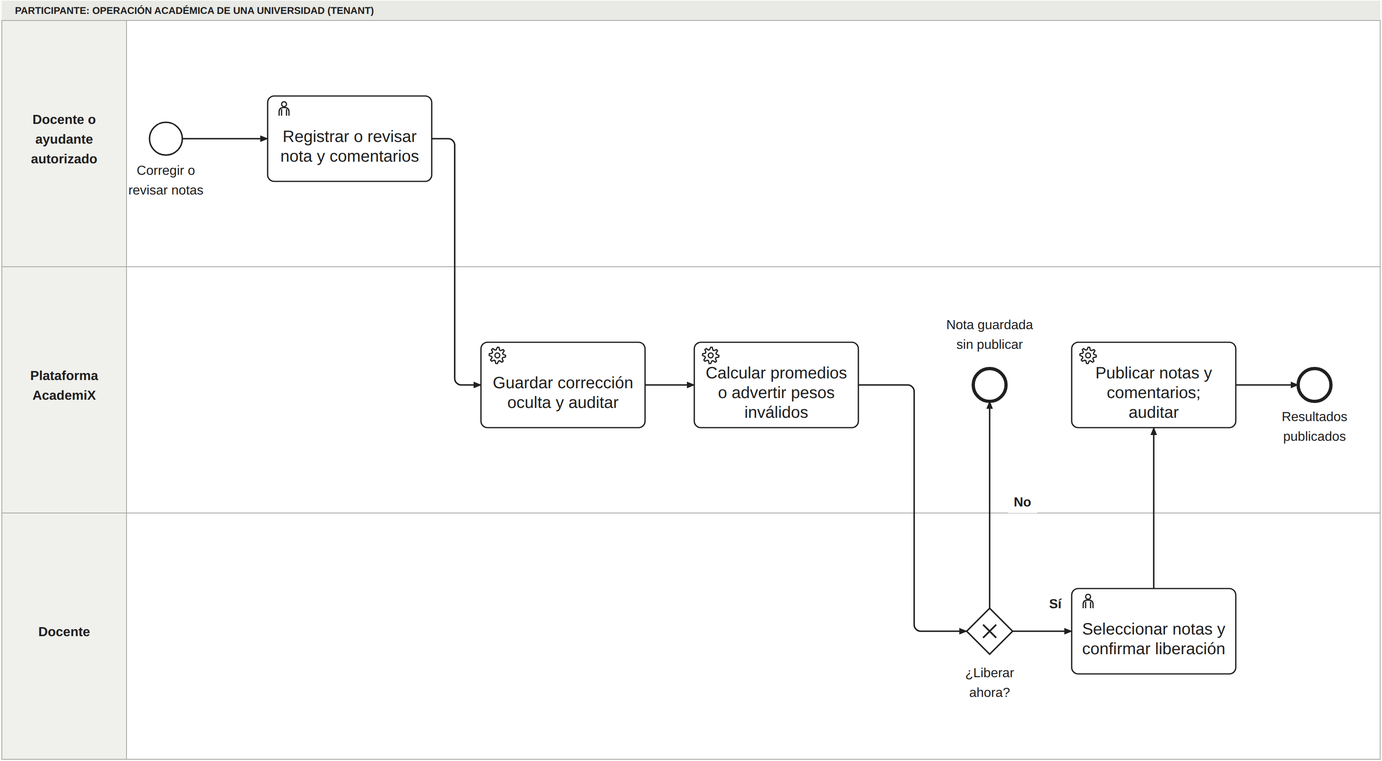
\includegraphics[width=\textwidth]{images/bpmn-03-teaching-correction-publication.png}
\end{column}
\begin{column}{0.35\textwidth}
\small
\textbf{Docente y ayudante autorizado.}
\begin{itemize}
  \item Registrar o revisar notas y comentarios.
  \item Guardar la corrección oculta y auditar los cambios.
  \item Calcular promedios o advertir ponderaciones inválidas.
  \item El docente decide cuándo liberar las notas.
\end{itemize}
\end{column}
\end{columns}
\end{frame}

\begin{frame}{Modelos de Proceso: Actividad del estudiante}
\begin{columns}[T,onlytextwidth]
\begin{column}{0.62\textwidth}
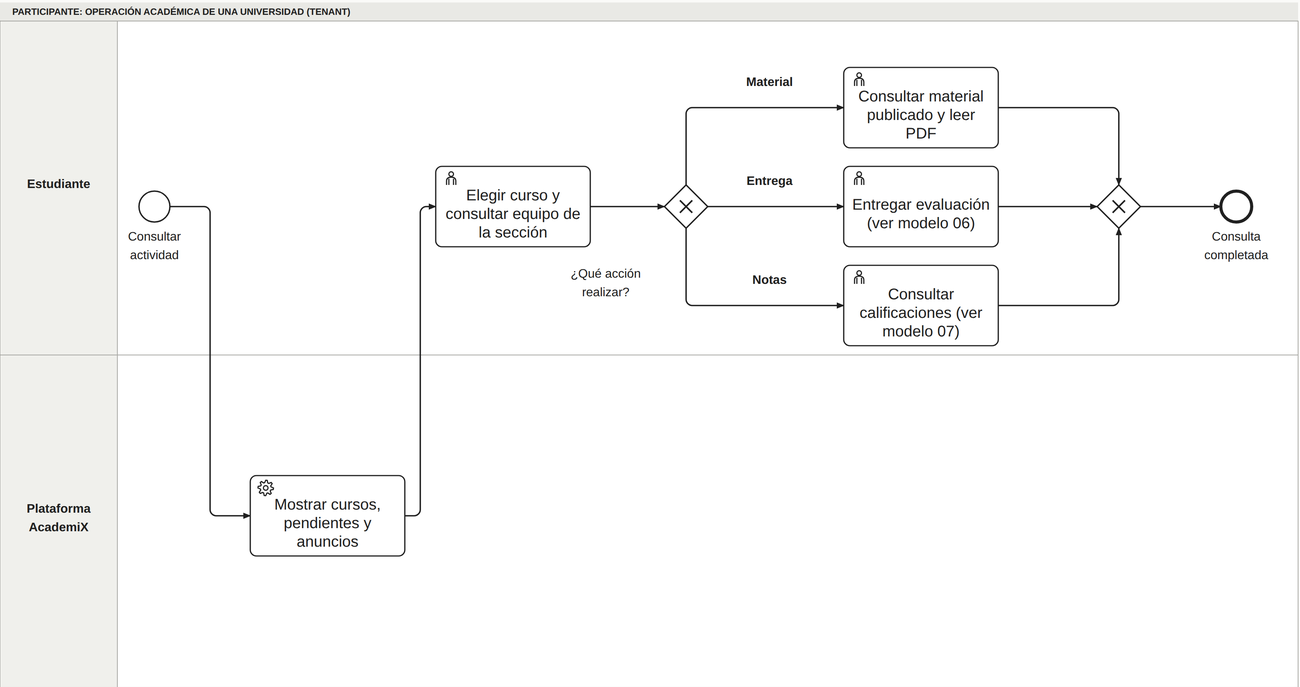
\includegraphics[width=\textwidth]{images/bpmn-05-student-activity.png}
\end{column}
\begin{column}{0.35\textwidth}
\small
\textbf{Consulta de la actividad académica.}
\begin{itemize}
  \item Ver cursos, pendientes y anuncios.
  \item Elegir un curso y consultar el equipo de la sección.
  \item Acceder al material publicado y leer PDF.
  \item Entregar evaluaciones o consultar calificaciones.
\end{itemize}
\end{column}
\end{columns}
\end{frame}

\begin{frame}{Modelos de Proceso: Entrega del estudiante}
\begin{columns}[T,onlytextwidth]
\begin{column}{0.62\textwidth}
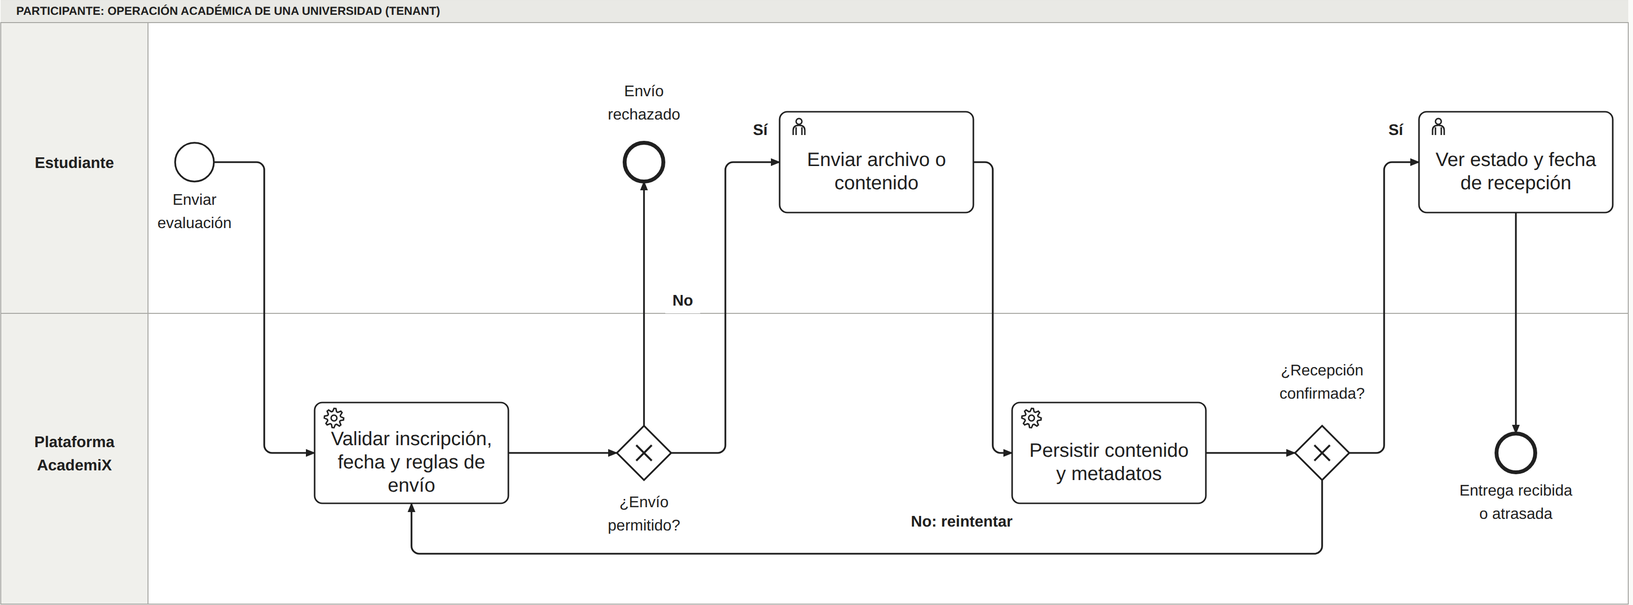
\includegraphics[width=\textwidth]{images/bpmn-06-student-delivery.png}
\end{column}
\begin{column}{0.35\textwidth}
\small
\textbf{Envío y confirmación de recepción.}
\begin{itemize}
  \item Validar inscripción, fecha y reglas de envío.
  \item Enviar el archivo o contenido si está permitido.
  \item Persistir contenido y metadatos; reintentar si no se confirma la recepción.
  \item Consultar el estado y la fecha de recepción.
\end{itemize}
\end{column}
\end{columns}
\end{frame}


% --- 4. Riesgos (60 s) ---
\begin{frame}{4. Riesgos y mitigaciones}
\footnotesize
\begin{tabularx}{\textwidth}{llYY}
\toprule
\textbf{Tipo} & \textbf{Riesgo} & \textbf{Impacto} & \textbf{Mitigación} \\
\midrule
Desarrollo & Sobrealcance & No llegar al MVP & Fundaciones \emph{must have} primero; extensiones sólo una vez validadas \\
Desarrollo & Multi-tenancy & Fuga o mezcla de datos & Registry, estructura idéntica por tenant y pruebas de acceso cruzado \\
Desarrollo & Grupos de estudiantes & Cambiar el modelo de entregas a mitad de camino & Entregas individuales hasta especificar membresías y autoría \\
Desarrollo & Carga en ventanas críticas & Fallas en cierres de entrega & Consultas eficientes y réplicas stateless; pool, caché y workers con justificación \\
Desarrollo & Archivos & Saturación y costo de la base & Binarios en object storage; metadatos en PostgreSQL \\
Negocio & Crédito cloud agotado & Perder el ambiente público antes del cierre & Crédito acotado al proyecto, escala a cero y límites declarados \\
Negocio & Competencia LMS & Diferencial difuso & Foco en flujo integrado y transparencia de calificaciones \\
Negocio & Baja adopción & Vuelta a planillas y carpetas & Cada vista nace de una historia con criterios de aceptación \\
Negocio & IA prematura & Costo y distracción del core & Posterior al core, acotada al material publicado, con citas \\
\bottomrule
\end{tabularx}
\end{frame}

% --- 5a. Alcance y RF (70 s) ---
\begin{frame}[t]{5. Solución: alcance funcional y trazabilidad}
\footnotesize
\vspace{0.15cm}
\begin{tabularx}{\textwidth}{lYl}
\toprule
\textbf{Bloque} & \textbf{Resultado para el usuario} & \textbf{RF / Historias} \\
\midrule
Tenant, permisos y cuerpo docente & Universidad aislada, roles por tenant y curso, equipo docente visible & RF1--RF5, RF21 / US5--US8, US30 \\
Contenido & Módulos, material y visibilidad controlada & RF6--RF8 / US9--US12 \\
Evaluaciones y entregas & Fecha, puntaje, evidencia de envío y estado & RF9--RF12 / US13--US16 \\
Cálculo, corrección y notas & Promedios por ponderación, comentarios, liberación y libro de notas & RF13--RF16, RF19, RF22 / US17--US21 \\
Dashboard y anuncios & Pendientes y comunicación del curso & RF18 / US1--US4, US23, US24 \\
\midrule
Extensiones del core & Lector de PDF, recorrección y calendario interno & RF20, RF17, RFO5 / US26, US22, US25 \\
\emph{Nice to have} & Video, resumen con IA, chats y alertas internas & RFO1--RFO4, RFO6 / US27--US29, US31--US36 \\
\bottomrule
\end{tabularx}
\vspace{0.15cm}

{\footnotesize \st{Criterio:} fundaciones primero --- cursos, secciones, participantes, evaluaciones y calificaciones. Fuera del MVP: Google Calendar, Outlook, quizzes en vivo y alertas por correo (US37).}
\end{frame}

% --- 5b. RNF (70 s) ---
\begin{frame}[t]{5. Solución: RNF como atributo, acción y evidencia}
\small
\vspace{0.2cm}
\begin{tabularx}{\textwidth}{lYY}
\toprule
\textbf{Atributo} & \textbf{Acción de diseño / mitigación} & \textbf{Evidencia verificable} \\
\midrule
Aislamiento & Tenant resuelto por request contra el registry; base de datos por tenant & Escenario de acceso cruzado: la operación se bloquea \\
Seguridad & Roles contextuales: TenantMembership y CourseMembership & Casos de permiso por rol y por curso \\
Auditabilidad & Actor, fecha, valor anterior y nuevo en notas y liberaciones & Reconstruir el historial de una nota \\
Integridad & Recepción confirmada sólo con archivo y metadatos persistidos & Subida fallida que no deja entrega ni nota inválida \\
Disponibilidad & Despliegue reproducible, logs y redespliegue; balanceo con varias réplicas & Escenario de caída parcial y monitoreo en cierres \\
Rendimiento & Consultas, índices y medición de endpoints antes de introducir caché & Medición de dashboard y curso como condición previa \\
Escalabilidad & Réplicas stateless; el tenant es el shard; réplica de lectura por tenant & Spike de $\sim$1.000 concurrentes como caso de diseño \\
\bottomrule
\end{tabularx}
\vspace{0.15cm}
{\footnotesize En vez de metas numéricas prematuras, la documentación fija escenarios de calidad: qué falla probable enfrentamos y cómo reacciona el sistema.}
\end{frame}

% --- 5c. Stack y decisiones abiertas (60 s) ---
\begin{frame}[t]{5. Solución: stack, proveedor y decisiones abiertas}
\small
\vspace{0.15cm}
\begin{columns}[T,onlytextwidth]
\begin{column}{0.52\textwidth}
\begin{itemize}
  \item \st{Stack:} Next.js (cliente web), NestJS (monolito modular), PostgreSQL (notas y estados transaccionales), Docker.
  \item \st{Proveedor:} GCP por su crédito de USD 300 por 3 meses --- Cloud Run, Cloud SQL, Cloud Storage. Componentes portables a otro proveedor.
  \item \st{Condicional:} balanceador con más de una réplica; PgBouncer si las conexiones presionan Cloud SQL.
  \item \st{En veremos:} Redis y workers entran juntos, atados a US concretas (archivos, recálculo de promedios, notificaciones).
\end{itemize}
\end{column}
\begin{column}{0.45\textwidth}
\begin{block}{Decisiones abiertas}
\footnotesize
\begin{itemize}
  \item Umbrales de rendimiento: se fijan midiendo, y la medición decide si entra caché.
  \item Activación de Redis y workers: al especificar la US que los justifique.
  \item Grupos de estudiantes: sin especificación, el modelo sigue individual.
  \item Qué extensiones \emph{nice to have} entran, según avance.
  \item Modelo y costo del asistente de IA.
  \item Estrategia de base de datos.
\end{itemize}
\end{block}
\end{column}
\end{columns}
\end{frame}

% --- 5d. Arquitectura (50 s) ---
\begin{frame}{5. Solución: primera versión de la arquitectura}
\centering
\resizebox{0.97\textwidth}{!}{%
\begin{tikzpicture}[
  font=\sffamily\footnotesize,
  base/.style={draw=academixnavy,thick,fill=academixbg,rounded corners=2pt,align=center,inner sep=3pt,text width=2.6cm},
  cond/.style={draw=academixamber,thick,dashed,fill=white,rounded corners=2pt,align=center,inner sep=3pt,text width=2.6cm},
  maybe/.style={draw=academixslate,thick,dotted,fill=white,rounded corners=2pt,align=center,inner sep=3pt,text width=2.6cm},
  fl/.style={-{Latex[length=1.8mm]},draw=academixnavy,thick},
  fld/.style={-{Latex[length=1.8mm]},draw=academixamber,thick,dashed},
  flm/.style={-{Latex[length=1.8mm]},draw=academixslate,thick,dotted},
]
\node[base] (u) at (0,0) {\textbf{Usuarios}\\estudiante · docente\\ayudante · admin};
\node[base] (fe) at (3.6,0) {\textbf{Next.js}\\frontend web\\Cloud Run};
\node[base,text width=3.2cm] (be) at (7.5,0) {\textbf{NestJS modular}\\Cloud Run\\Auth JWT · Tenant Resolver};
\node[cond] (lb) at (5.55,1.9) {\textbf{Load balancer}\\API gateway};
\node[base] (treg) at (11.6,1.9) {\textbf{Tenant Registry}\\PostgreSQL central\\subdominio $\rightarrow$ config};
\node[cond] (cp) at (11.6,0) {\textbf{Connection pool}\\PgBouncer};
\node[base,text width=3.0cm] (db) at (15.4,0) {\textbf{PostgreSQL por tenant}\\Cloud SQL\\1 shard = 1 tenant};
\node[base] (gcs) at (11.6,-1.9) {\textbf{Cloud Storage}\\material y entregas};
\node[maybe] (redis) at (11.6,-3.6) {\textbf{Redis}\\cola y caché};
\node[maybe] (wk) at (15.4,-3.6) {\textbf{Workers}\\fuera del request};
\draw[fl] (u) -- (fe);
\draw[fl] (fe) -- (be);
\draw[fld] (fe) |- (lb);
\draw[fld] (lb) -| (be);
\draw[fl] (be) |- (treg);
\draw[fld] (be) -- (cp);
\draw[fl] (cp) -- (db);
\draw[fl] (be) |- (gcs);
\draw[flm] (be) |- (redis);
\draw[flm] (redis) -- (wk);
\node[align=left,font=\sffamily\scriptsize] at (3.4,-3.6) {%
\textcolor{academixnavy}{\textbf{---}}~base, desde el primer despliegue\\
\textcolor{academixamber}{\textbf{-- --}}~condicional, al desplegar o con carga\\
\textcolor{academixslate}{\textbf{$\cdots$}}~en veremos, atado a una historia};
\end{tikzpicture}}\\
\vspace{0.1cm}
{\footnotesize Monolito modular primero. Los tenant comienzan aislados.  Y el tenant es el shard desde el primer despliegue.}
\end{frame}

% --- 5e. Maquetas (50 s) ---
\begin{frame}{5. Solución: primeras maquetas}
\centering
\setlength{\tabcolsep}{3pt}
\begin{tabular}{ccc}
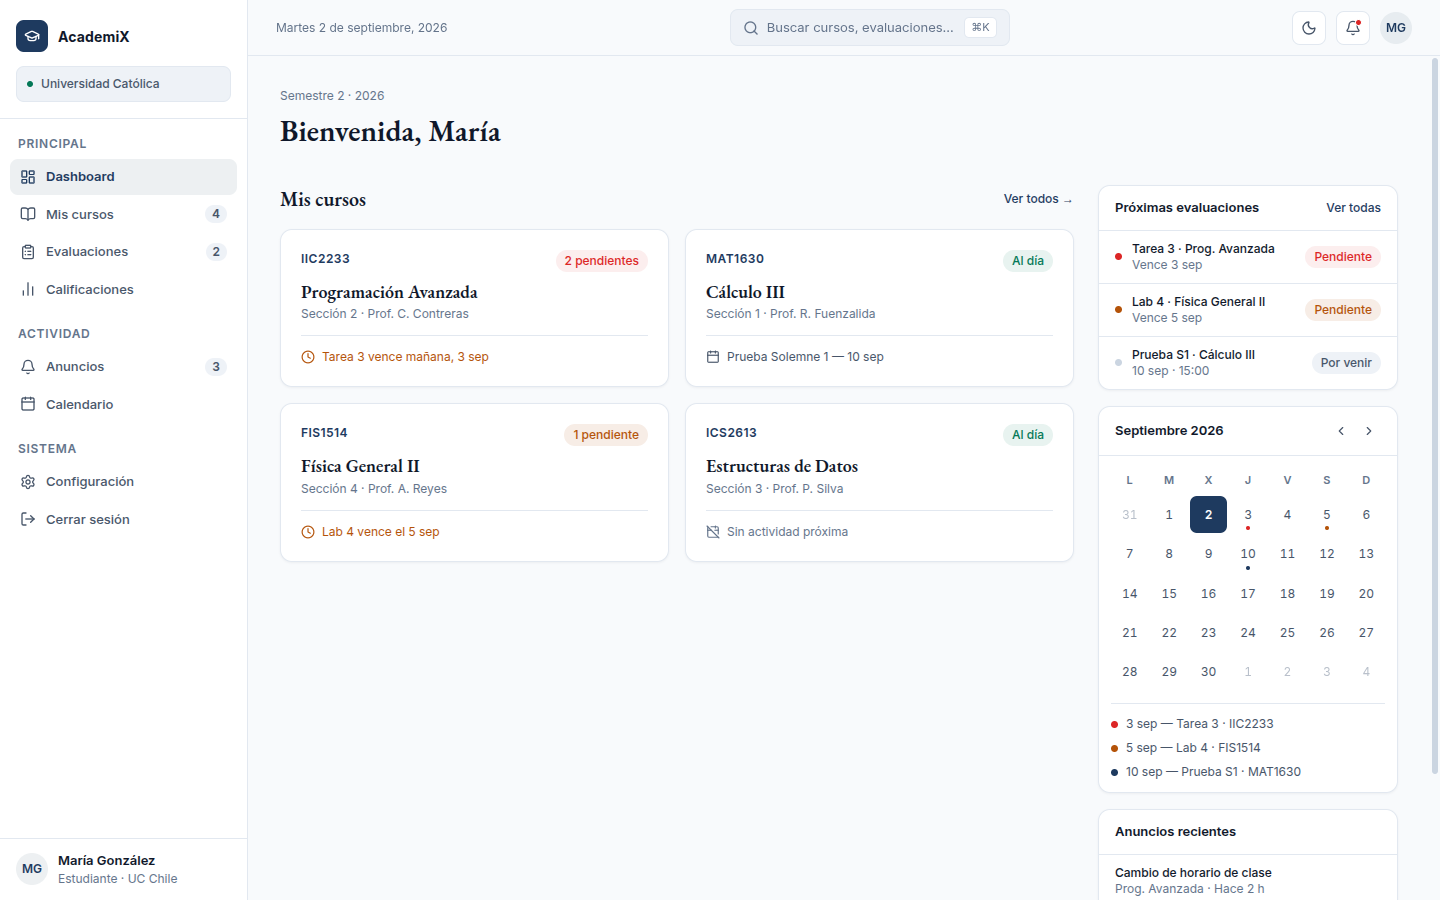
\includegraphics[width=0.31\textwidth]{images/mockup-dashboard.png} &
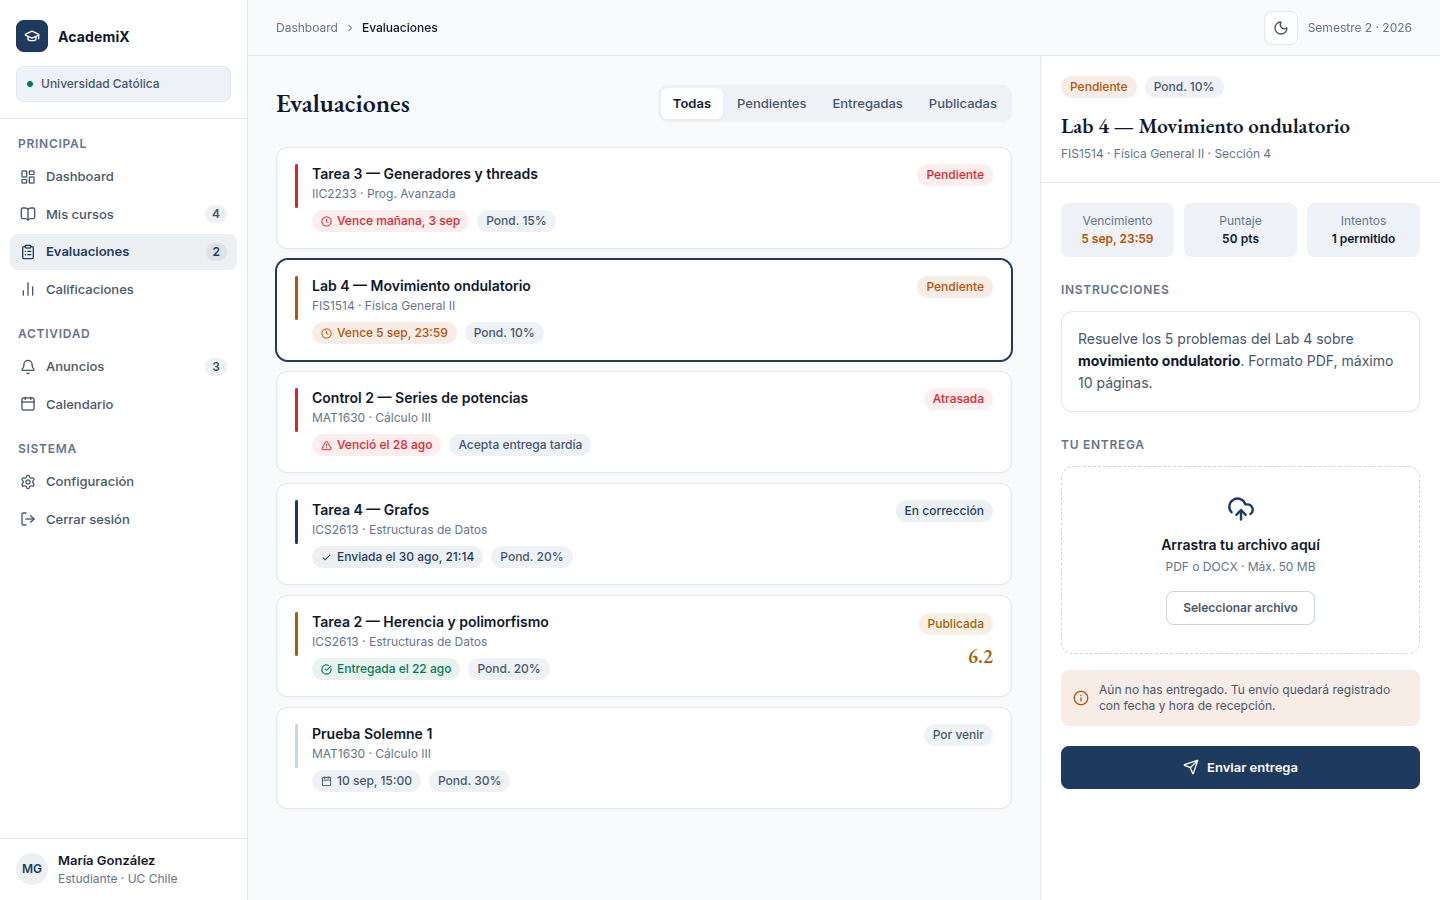
\includegraphics[width=0.31\textwidth]{images/mockup-evaluations.png} &
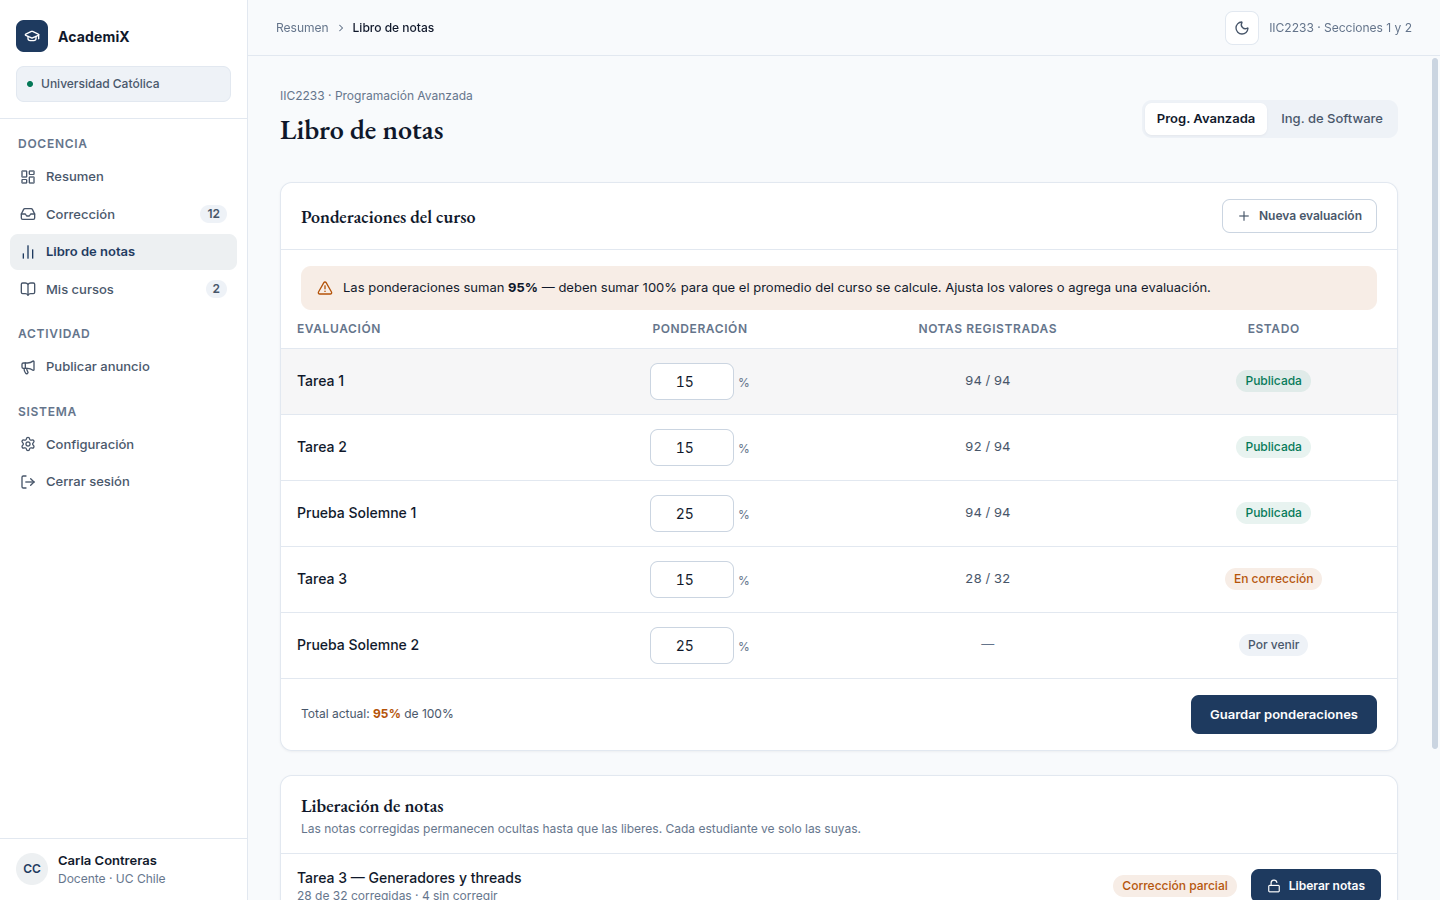
\includegraphics[width=0.31\textwidth]{images/mockup-teacher-gradebook.png} \\
{\footnotesize Dashboard estudiante} & {\footnotesize Evaluaciones y entrega} & {\footnotesize Libro de notas docente} \\
{\scriptsize US1--US3, US24, US25} & {\scriptsize US13--US16, US21} & {\scriptsize US17, US18} \\
\end{tabular}
\vspace{0.25cm}

{\footnotesize Mockups navegables en HTML estático. Notas del estudiante, panel docente y lector de PDF quedan en los anexos.}
\end{frame}

% --- 6. Plan (50 s) ---
\begin{frame}{6. Plan de trabajo: 12 iteraciones semanales}
\small
\begin{tabularx}{\textwidth}{lYY}
\toprule
\textbf{Sem.} & \textbf{Actividades técnicas (RF/RNF)} & \textbf{No técnicas y estado esperado} \\
\midrule
1--2 & Monorepo, autenticación y tenancy (RF1, RF2, RNF3, RNF4) & Visión, arquitectura, maquetas y backlog: tenant resuelto en cada request \\
3--4 & Cursos, secciones, participantes, cuerpo docente, módulos y material (RF3--RF8, RF20, RF21) & Validación de maquetas: un curso real con material publicado \\
5--7 & Evaluaciones, entregas, corrección y liberación (RF9--RF13, RF16) & Criterios de aceptación y revisión entre pares: ciclo completo funcionando \\
8--9 & Libro de notas, promedios, auditoría, dashboard y anuncios (RF14, RF15, RF18, RF19, RF22) & Demo intermedia: docente y estudiante ven el mismo contenido \\
10--11 & Despliegue en GCP, observabilidad, permisos y pruebas (RNF1--RNF4, RNF6, RNF9, RNF10) & ADR de decisiones abiertas: ambiente público operativo \\
12 & Deuda crítica y ajustes de UX & Demo final, documentación y presentación \\
\bottomrule
\end{tabularx}
\vspace{0.1cm}
% {\footnotesize Ventana efectiva de 10 a 12 semanas: las iteraciones 11 y 12 son colchón de cierre y pueden comprimirse.}
\end{frame}

% --- Cierre (30 s) ---
\begin{frame}{Cierre}
\begin{block}{Propuesta}
AcademiX es un LMS universitario multi-tenant enfocado en integrar el flujo académico crítico del curso semestral, con calificaciones transparentes y aislamiento por institución.
\end{block}
\begin{itemize}
  \item \textbf{Valor:} claridad para el estudiante, control para el cuerpo docente, aislamiento para la institución.
  \item \textbf{Fundaciones:} cursos y secciones, participantes, cuerpo docente visible, evaluaciones y calificaciones.
  \item \textbf{Camino:} iteraciones semanales, fundaciones primero, extensiones sólo con evidencia de avance.
\end{itemize}
\vspace{0.2cm}
\centering\small ¿Preguntas?
\end{frame}

\appendix

% --- Respaldo para preguntas ---
\begin{frame}{Anexo: escala objetivo y escenarios de calidad}
\small
\begin{columns}[T,onlytextwidth]
\begin{column}{0.45\textwidth}
\begin{block}{Supuestos de escala}
\footnotesize
\begin{itemize}
  \item Hasta 5 universidades.
  \item Hasta 30.000 estudiantes por universidad (150.000 potenciales).
  \item Spikes de $\sim$1.000 concurrentes en ventanas de evaluación, entrega o publicación.
  \item Estos supuestos orientan a la arquitectura
\end{itemize}
\end{block}
\end{column}
\begin{column}{0.52\textwidth}
\begin{block}{Escenarios de calidad}
\footnotesize
\begin{itemize}
  \item Dashboard lento en carga normal.
  \item Spike durante evaluaciones o entregas.
  \item Falla al subir una entrega.
  \item Caída parcial de una instancia.
  \item Intento de acceso cruzado entre tenants.
  \item Cambio de nota, ponderación o liberación.
  \item Restauración por error operativo.
\end{itemize}
\end{block}
\end{column}
\end{columns}
\end{frame}

\begin{frame}{Anexo: glosario mínimo}
\small
\begin{tabularx}{\textwidth}{lY}
\toprule
\textbf{Término} & \textbf{Definición} \\
\midrule
Tenant & Universidad aislada dentro de la plataforma. \\
Tenant registry & Base central que resuelve el subdominio a la configuración del tenant. \\
Shard & Partición de datos; aquí un shard equivale a un tenant desde el inicio. \\
Curso & Ramo semestral concreto de un periodo académico. \\
Evaluación & Actividad con entrega, corrección, nota y ponderación. \\
Liberación de notas & Acción del docente que hace visible una nota. \\
Libro de notas & Vista consolidada de evaluaciones, ponderaciones, notas y promedio. \\
Rol contextual & Rol que depende del tenant y del curso, no del usuario global. \\
Escenario de calidad & Falla probable descrita junto a la reacción esperada del sistema. \\
RFO & Requisito funcional opcional, condicionado al avance del proyecto. \\
\bottomrule
\end{tabularx}
\end{frame}

\begin{frame}{Anexo: trazabilidad RF $\rightarrow$ historias}
\small
\begin{columns}[T,onlytextwidth]
\begin{column}{0.49\textwidth}
RF1 habilitador · RF2 US5, US8, US12, US30 · RF3 US5 · RF4 US5, US6 · RF5 US7, US8 · RF6 habilitador · RF7 US9, US10 · RF8 US11, US12 · RF9 US13, US17 · RF10 US2, US16 · RF11 US14 · RF12 US15
\end{column}
\begin{column}{0.49\textwidth}
RF13 US18 · RF14 US19, US20 · RF15 US17, US19, US20 · RF16 US15, US21 · RF17 US22 · RF18 US1--US4, US23, US24 · RF19 habilitador (auditoría) · RF20 US26 · RF21 US30 · RF22 US17, US20 · RFO1--RFO7 US31--US37 y US25
\end{column}
\end{columns}
\vspace{0.3cm}
{\footnotesize Las 37 historias tienen criterios de aceptación y prioridad MoSCoW. RF1, RF6 y RF19 son habilitadores transversales: se validan a través de las historias de los bloques que los usan.}
\end{frame}

\begin{frame}{Anexo: vista de notas del estudiante}
\begin{columns}[T,onlytextwidth]
\begin{column}{0.62\textwidth}
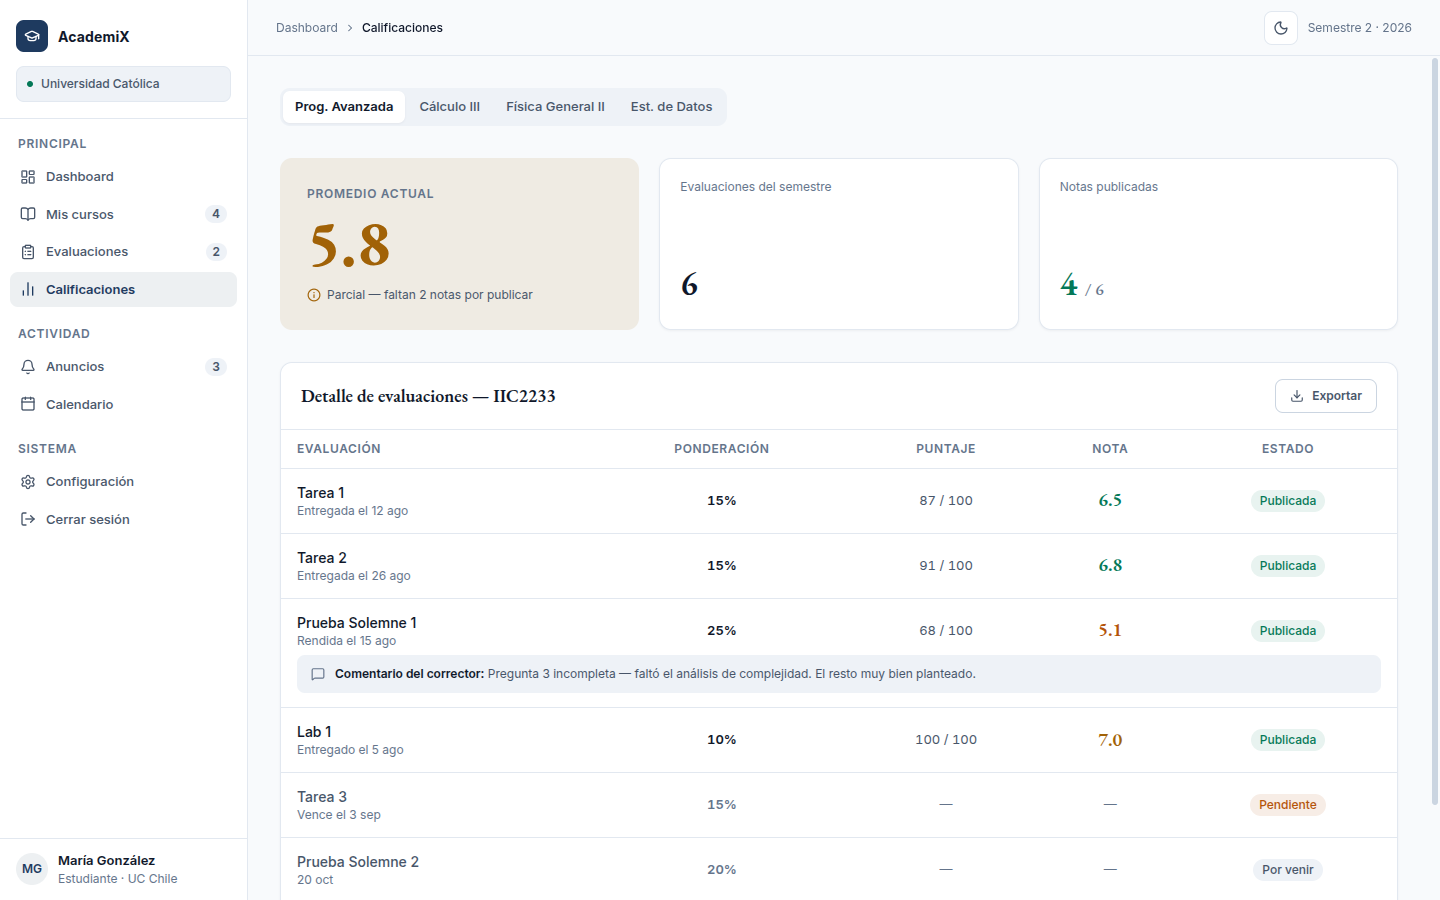
\includegraphics[width=\textwidth]{images/mockup-grades.png}
\end{column}
\begin{column}{0.35\textwidth}
\small
\textbf{Fundación \emph{must have} (US17--US20).}
\begin{itemize}
  \item Sólo notas liberadas por el docente.
  \item Ponderación visible por evaluación.
  \item Promedio parcial con advertencia explícita.
  \item Comentario del corrector junto a la nota.
\end{itemize}
\end{column}
\end{columns}
\end{frame}

\begin{frame}{Anexo: panel del docente}
\begin{columns}[T,onlytextwidth]
\begin{column}{0.62\textwidth}
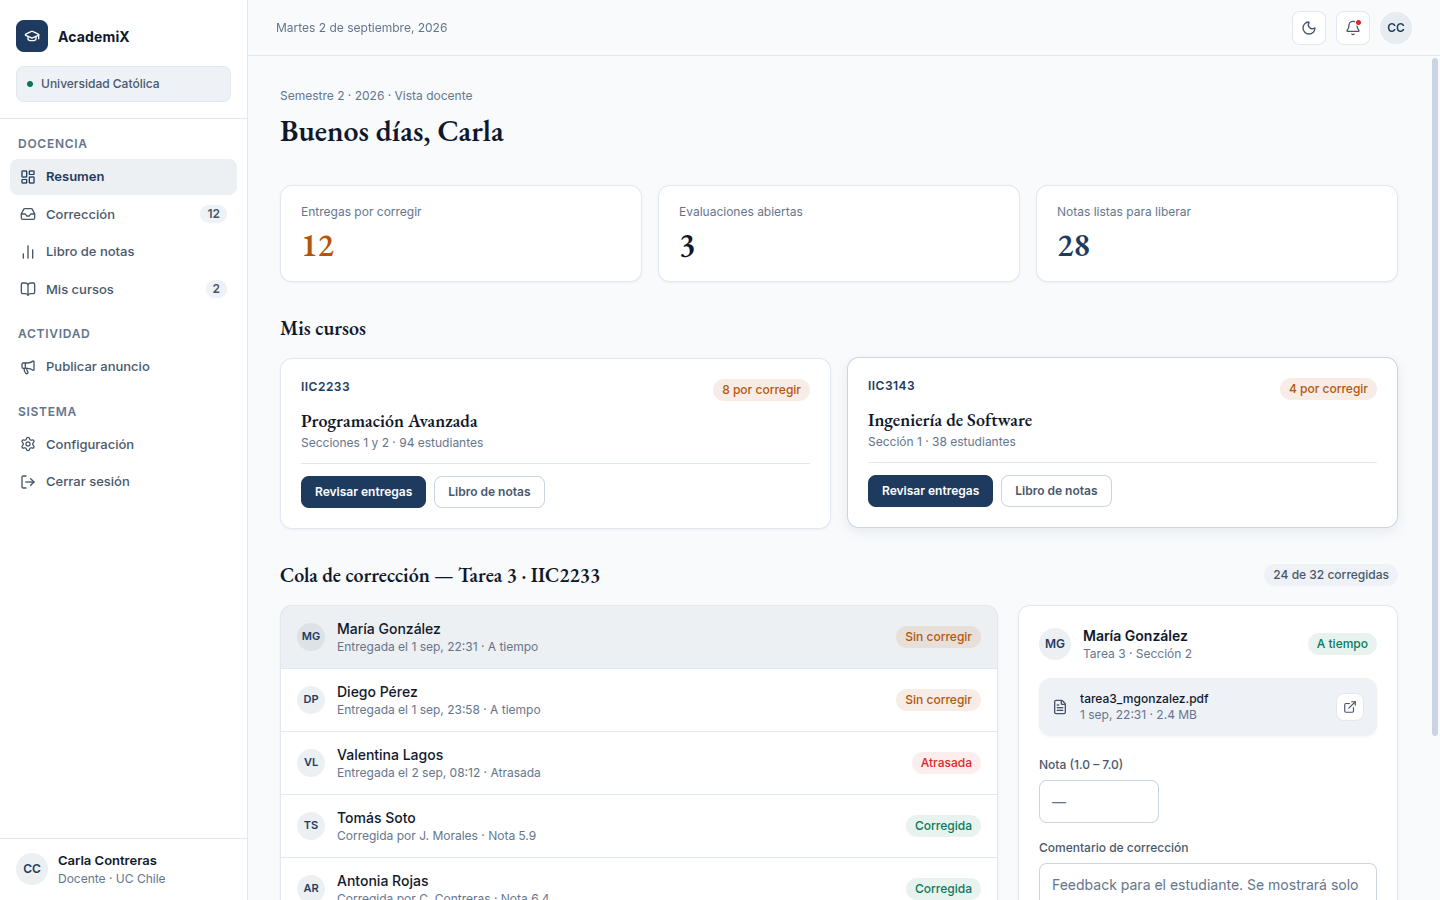
\includegraphics[width=\textwidth]{images/mockup-teacher-dashboard.png}
\end{column}
\begin{column}{0.35\textwidth}
\small
\textbf{Should have (US4, US15, US21).}
\begin{itemize}
  \item Entregas por corregir agrupadas por curso.
  \item Corrección con nota y comentario.
  \item Sin publicación automática al estudiante.
  \item Sólo cursos donde el usuario es docente o ayudante autorizado.
\end{itemize}
\end{column}
\end{columns}
\end{frame}

\begin{frame}{Anexo: lector de PDF y asistente de IA}
\begin{columns}[T,onlytextwidth]
\begin{column}{0.62\textwidth}
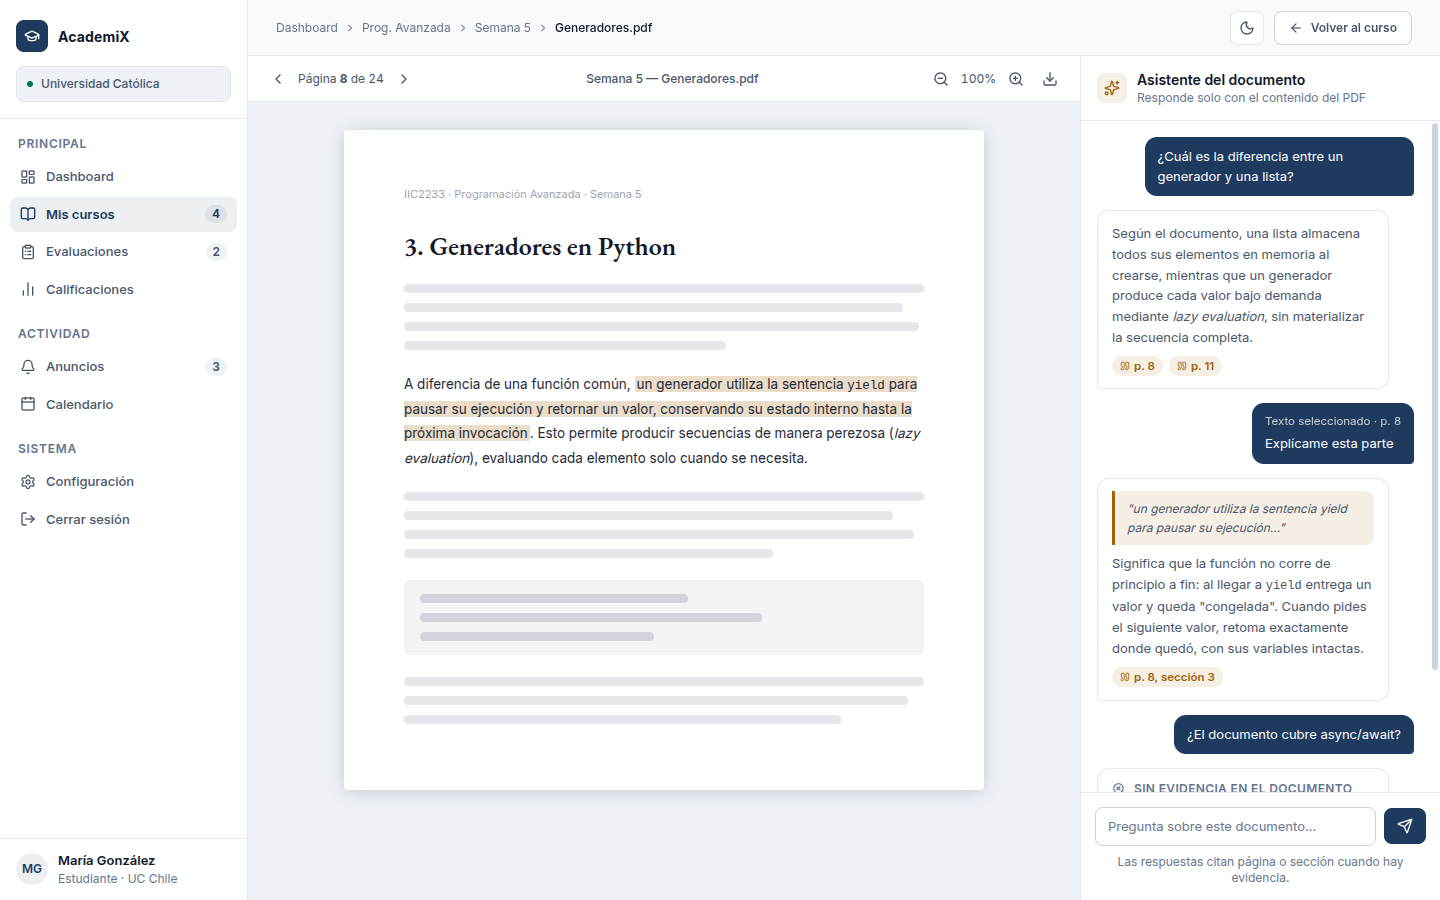
\includegraphics[width=\textwidth]{images/mockup-pdf-reader.png}
\end{column}
\begin{column}{0.35\textwidth}
\small
\textbf{Lector de PDF: should have (US26).}\\
\textbf{Asistente de IA: could have (US27--US29).}
\begin{itemize}
  \item Lectura del material sin descargar archivos.
  \item Preguntas acotadas al documento abierto.
  \item Respuestas con cita de página o sección.
  \item Caso explícito de respuesta sin evidencia.
\end{itemize}
\vspace{0.1cm}
{\footnotesize Ninguna de las dos bloquea las fundaciones.}
\end{column}
\end{columns}
\end{frame}

\end{document}
